\documentclass[12pt]{article}
\usepackage[utf8]{inputenc}
\usepackage{graphicx} % Allows you to insert figures
\usepackage{subcaption}
\usepackage{amsmath} % Allows you to do equations
\usepackage{fancyhdr} % Formats the header
\usepackage{geometry} % Formats the paper size, orientation, and margins
\usepackage{dirtytalk} % typesetting different types of quotation
\usepackage[english]{babel}
\usepackage{csquotes}
\usepackage{hyperref}
\usepackage{listings}
\lstset{
    language=C,
    basicstyle=\ttfamily, 
    numberstyle=\tiny,
    basicstyle=\small,
    frame=single,
    breaklines=true,
    stepnumber=1,                   % the step between two line-numbers.        
    tabsize=2,                      % sets default tabsize to 2 spaces
    breaklines=true,                % sets automatic line breaking
    breakatwhitespace=true,         % sets if automatic breaks should only happen at whitespace
    title=pseudocode
}

\linespread{1.25} % About 1.5 spacing in Word
\setlength{\parindent}{0.8cm} % No paragraph indents
\setlength{\parskip}{0em} % Paragraphs separated by one line
\renewcommand{\headrulewidth}{0pt} % Removes line in header
\geometry{a4paper, portrait, margin=1in}
\setlength{\headheight}{14.49998pt}
\graphicspath{ {images/} }

\begin{document}
\begin{titlepage}
   \begin{center}
    \textsc{\large Ministry of Education of Republic of Moldova}\\[0.5cm]
    \textsc{\large Technical University of Moldova}\\[0.5cm]
    \textsc{\large Faculty of Computers, Informatics and Microelectronics}\\[0.5cm]
    \textsc{\large Software Engineering Department}\\[1.2cm]
    
    \vspace{25 mm}
    
    \textsc{\Large Computer Programming}\\[0.5cm]
    \textsc{\large Laboratory work \#4}\\[0.5cm]    % <<<<<<< CHANGE LAB NUMBER HERE
    
    \newcommand{\HRule}{\rule{\linewidth}{0.5mm}}
    \vspace{10 mm}
    \HRule \\[0.4cm]
    { \LARGE \bfseries Character and String Operations }\\[0.4cm] % <<<<<<< CHANGE LAB TITLE HERE
    \HRule \\[1.5cm]
    
    \vspace{10mm}
    
    \begin{minipage}[t]{0.4\textwidth}
    \begin{flushleft} \large
    \emph{Author:} \\
    Andrei \textsc{Chicu}\\                         % <<<<<<< CHANGE YOUR NAME HERE
    std. gr. FAF-233                                % <<<<<<< CHANGE GROUP NUMBER HERE
    \end{flushleft}
    \end{minipage}
    ~
    \begin{minipage}[t]{0.4\textwidth}
    \begin{flushright} \large
    \emph{Verified:} \\
    Alexandru \textsc{Furdui}\\
    \end{flushright}
    \end{minipage}\\[3cm]
    
    \vspace{5 mm}
    \large Chișinău 2023\\[0.5cm]
    
    \vfill
    \end{center}
\end{titlepage}

\setcounter{page}{2}
\pagestyle{fancy}
\fancyhf{}
\rhead{\thepage}
\lhead{FAF-233 Andrei Chicu; Laboratory Work №4}

% \section*{Introduction}
\section*{Theory Background}
In C, a string is a sequence of characters stored as an array of characters. It is terminated by a null character \texttt{\ 0}, which marks the end of the string. Strings in C are commonly represented as character arrays, where each element of the array corresponds to a character in the string, and the null character signifies the string's endpoint.

The program for this laboratory work defines a buffer structure to manage the text data and a set of functions for operations like reading from and writing to files, searching for words, and replacing words within the text buffer and offers a text-based user interface for interacting with these features, allowing users to perform various text manipulation tasks.

\section*{The Task}

Describe your task, and enumerate the task/tasks you have implemented:

\textbf{Task Hard -- Text editor.}

\section*{Technical implementation}
The full code:\\
\url{https://github.com/andyp1xe1/pc_labs/tree/master/lab4}

\begin{lstlisting}
# Define delimiters
DELIM = " ,.!:;?\n\t\r"

# Define a buffer structure
buffer:
  size: size_t
  pos: size_t
  dat: char*

# Function to reallocate buffer memory
function realloc_buff(buff: buffer, scale: float):
  tmp = realloc(buff.dat, sizeof(char) * buff.size * scale)
  if tmp is not NULL:
    buff.dat = tmp
  else:
    print "Not all text was read, realloc error"

# Function to clear the buffer
function clear_buff(buff: buffer):
  free(buff.dat)
  buff.size = 2
  buff.pos = 0
  buff.dat = malloc(sizeof(char) * buff.size)

# Function to display the contents of the buffer
function display_buff(buff: buffer):
  if buff.pos > 0:
    print buff.dat
  else:
    print "Buffer is empty!"

# Function to search for and count occurrences of a word in the buffer
function search_n_count(word: char, buff: buffer) -> int:
  n = 0
  newstr = copy of buff.dat
  token = strtok(newstr, DELIM)
  while token is not NULL:
    if token is equal to word:
      n = n + 1
    token = strtok(NULL, DELIM)
  return n

# Function to check if a string contains any delimiter characters
function has_delim(str: char) -> bool:
  for i in range(0, length of str):
    for j in range(0, length of DELIM):
      if str[i] is equal to DELIM[j]:
        return true
  return false

# Function to substitute a word in the buffer with another word
function substitute_word_in_buff(in: char, re: char, buff: buffer):
  token = empty string
  str = copy of buff.dat
  newbuff.size = buff.size
  newbuff.dat = allocate memory for newbuff.size characters
  n = 0
  while n <= length of str:
    if str[n] is a delimiter character:
      if token is not empty:
        if token is equal to in:
          if length of re >= length of in:
            realloc_buff(newbuff, 1.5)
          append re to newbuff.dat
        else:
          append token to newbuff.dat
        token = empty string
      append str[n] to newbuff.dat
    else:
      append str[n] to token
    n = n + 1
  buff.dat = newbuff.dat
  buff.size = newbuff.size
  buff.pos = length of newbuff.dat
  free(token)
  free(str)

# Function to read text from a file into the buffer
function read_to_buff(buff: buffer, fd: FILE):
  i = buff.pos
  while character c from fd is not EOF:
    if buff.size is equal to i:
      realloc_buff(buff, 1.5)
    if i is not 0 or c is not newline character:
      buff.dat[i] = c
      i = i + 1
  if buff.dat[i - 1] is newline character:
    i = i - 1
  buff.dat[i] = null character
  buff.pos = i

# Function to read text from a file and append it to the buffer
function read_from_file_to_buff(path: char, buff: buffer):
  open the file at path in read mode and assign it to fd
  if fd is not NULL and no error occurred:
    read_to_buff(buff, fd)
    close the file fd
  else:
    print "Error"

# Function to write the buffer contents to a file
function write_from_buff_to_file(path: char, buff: buffer):
  open the file at path in write mode and assign it to fd
  if fd is not NULL and no error occurred:
    write the contents of buff.dat to fd
    close the file fd
  else:
    print "Error"

# Main REPL function
function repl(buff: buffer):
  print "Type 'h' for help message"
  loop:
    if stdin is at EOF:
      read a character from stdin and assign it to opt
    else:
      print "-> "
      read a string from stdin and assign it to opt
    switch opt:
      case 'h':
        print "h - Print this message"
        print "l - Clear console"
        print "d - Display text in buffer"
        print "i - Insert text and append to buffer"
        print "s - Substitute all occurrences of a word"
        print "c - Count all occurrences of a word"
        print "w - Write from buffer to file"
        print "r - Read from file and append to buffer"
        print "z - Clear buffer"
        print "! - End session"
      case 'l':
        clear the console
      case 'd':
        display_buff(buff)
      case 'i':
        print "Insert text to append:"
        read_to_buff(buff, stdin)
      case 's':
        read in and re
        if either in or re contains delimiter characters:
          print "One or both words are invalid"
        else:
          substitute_word_in_buff(in, re, buff)
      case 'c':
        print "Search term: "
        read a word into word
        n = search_n_count(word, buff)
        print n, " occurrences of ", word
      case 'w':
        print "File to write to: "
        read a file path into p
        write_from_buff_to_file(p, buff)
      case 'r':
        print "File to read from: "
        read a file path into p
        read_from_file_to_buff(p, buff)
      case 'z':
        clear_buff(buff)
        print "Buffer cleared!"
      case '!':
        print "Are you sure? It is recommended to save the buffer to a file before exiting (y/n): "
        read a character into o
        switch o:
          case 'y':
            exit with success
          default:
            break

# Main function
function main():
  create a buffer buff
  buff.size = 2
  buff.pos = 0
  buff.dat = allocate memory for buff.size characters
  call repl with buff as argument
  free buff.dat
  return 0
\end{lstlisting}

\section*{Results}
\hspace{0.8cm}
Here is a little showcase:

\begin{figure}[!h]
  \centering
  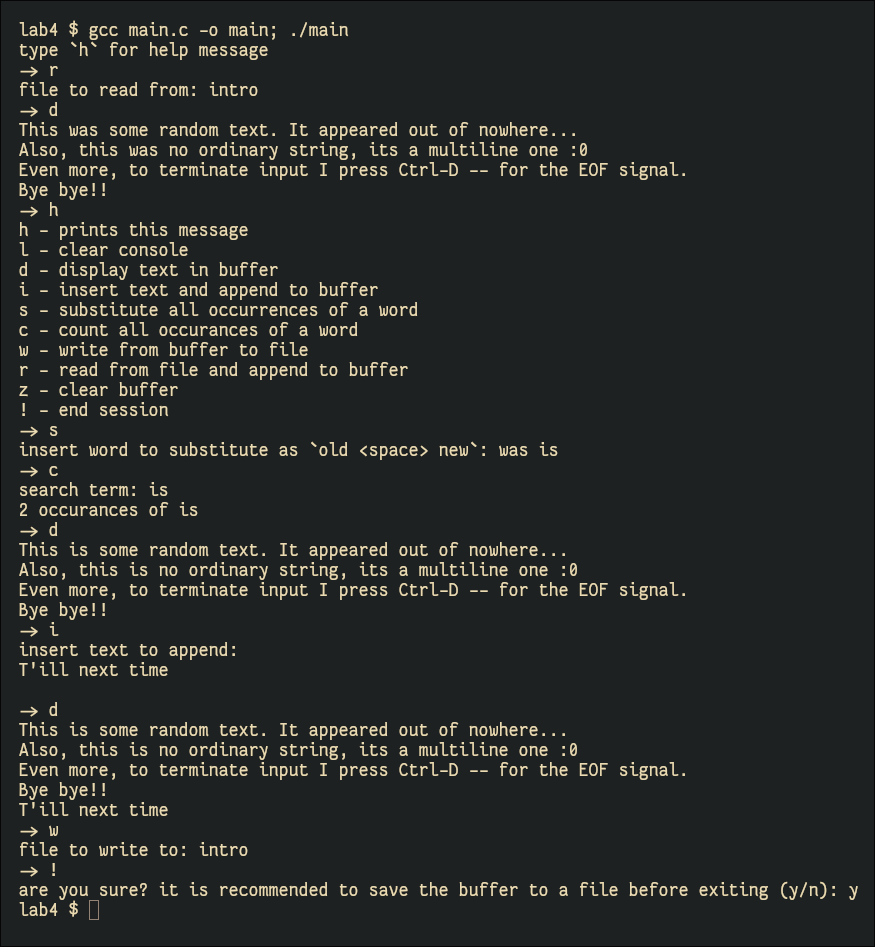
\includegraphics[width=6in]{texted.png}
  \caption{showcase}
\end{figure}

\section*{Conclusion}
\hspace{0.8cm}
The program I wrote serves as a basic text processing tool with features to manipulate text data interactively. It provides a simple command-line interface for users to perform operations such as appending text, searching for words, replacing words, and handling text files. While the code accomplishes these functions, there is room for improvement. For instance, it could benefit from better error handling and more user-friendly input validation. Additionally, the code might be enhanced by optimizing memory management, particularly when resizing the buffer and copying it at word replacement, to improve efficiency.

Overall, the code serves as a foundation for a text processing utility but can be further developed and refined for increased reliability and usability.

\section*{Refferences}
\hspace{0.8cm}
\begin{enumerate}
    \item \url{https://codebrowser.dev/glibc/glibc/string/strcmp.c.html}
    \item \url{https://www.geeksforgeeks.org/error-handling-during-file-operations-in-c-c/}
    \item \url{https://en.cppreference.com/w/c/experimental/dynamic/strdup}
    \item \url{https://www.geeksforgeeks.org/dynamic-memory-allocation-in-c-using-malloc-calloc-free-and-realloc/}
\end{enumerate}


\pagebreak
\end{document}
